%%=============================================================================
%% Results
%%=============================================================================

\chapter{\IfLanguageName{dutch}{Resultaten}{Results}}%
\label{ch:results}

The result section focuses on elaborating conducted experiments and acquired results. It specifies actual results, details about implementations and code snippet references.

\section{Jumper localization}
\label{results:jumper-localization}

% TODO: add, this is relevant
% TODO: convex hull the 3 jumpers and train on yolo model.
As DD3 routines are the focus of this research, the idea was to predict the coordinates and position of a team as a single unit, instead of individuals. This idea was supported by the fact that there aren't any public jump rope datasets and it was expected to increase the speed of labeling. The AI generated image \ref{fig:sr2-performance-ai-generated} shows an example of a competition setting where two athletes are performing a routine. The goal here would be to crop out the jumpers.

% TODO : add crop around jupers

Below you can find a shortlist of experiments executed on localization.

\begin{itemize}
    \item GoogleNet
    \item MobileNet
    % \item Vision Transformer
    \item YOLOv11
\end{itemize}

\subsection{Dedicated architectures}

This section explains the experiments using dedicated architectures. Results weren't good on about 6200 train and about 800 validation images. One issue might be that these models were finetuned for classification and not specialized for localization. A second issue might be the low amount of labels. Thirdly, predicting full boxes may not have been possible at all for the low amount of labels.
The first try-out used a personal implemenation, based on school courses of the GoogleNet architecture; \autocite{Szegedy2014} - \ref{code:keras-googlenet-small-replication}.
It used the an input shape of (Width, Height, Channels) to predict a full box around all three jumpers. Just like the implementation using MobileNetV3, \autocite{Howard2019} - \ref{code:keras-mobilenetv3small}.

% TODO Vision transformer?

Predictions only shifted a little towards the athletes, averaging out in the center of the image, reaching an IoU of about 28 to 30\%. These results where performed on the same dataset as in the experiment above.

\begin{itemize}
    \item MobileNet IoU unknown / lost
    \item GoogleNet IoU 31.06\%
    % \item Vision Transformer IoU 26.6\%
\end{itemize}

Predicting full teams didn't work out which allowed for a transition to labeling and predicting individuals athletes. Below you find more information about those experiments.

\subsection{YOLO}
\label{results:yolo}

Experiment 3, pre-trained models \& individual boxes.

The third experiment incorporates a double upgrade. The first upgrade involves annotating individual athletes on images instead of one big box around all jumpers. This method allows to annotate other routines such as single rope, chinese wheel or double dutch 4. The second upgrade is trying a pre-trained object detection model.

Ultralytics \autocite{Khanam2024} provides an easy-to-use pre-trained implementation for predicting people and objects in images which can be fine-tuned for specific use cases. Fine-tuning was needed as spectators, also humans, were also included in the predictions.

Using these predictions, a crop around the three jumpers can be created using the predicted jumper boxes from the fine-tuned YOLO model, after using the pre-trained weights on the COCO dataset \autocite{Lin2014}. In order to improve the crops some steps were required. Details are discussed below.

\subsubsection{Crop stability}
\label{results:crop-stability}

\begin{figure}
    \centering
    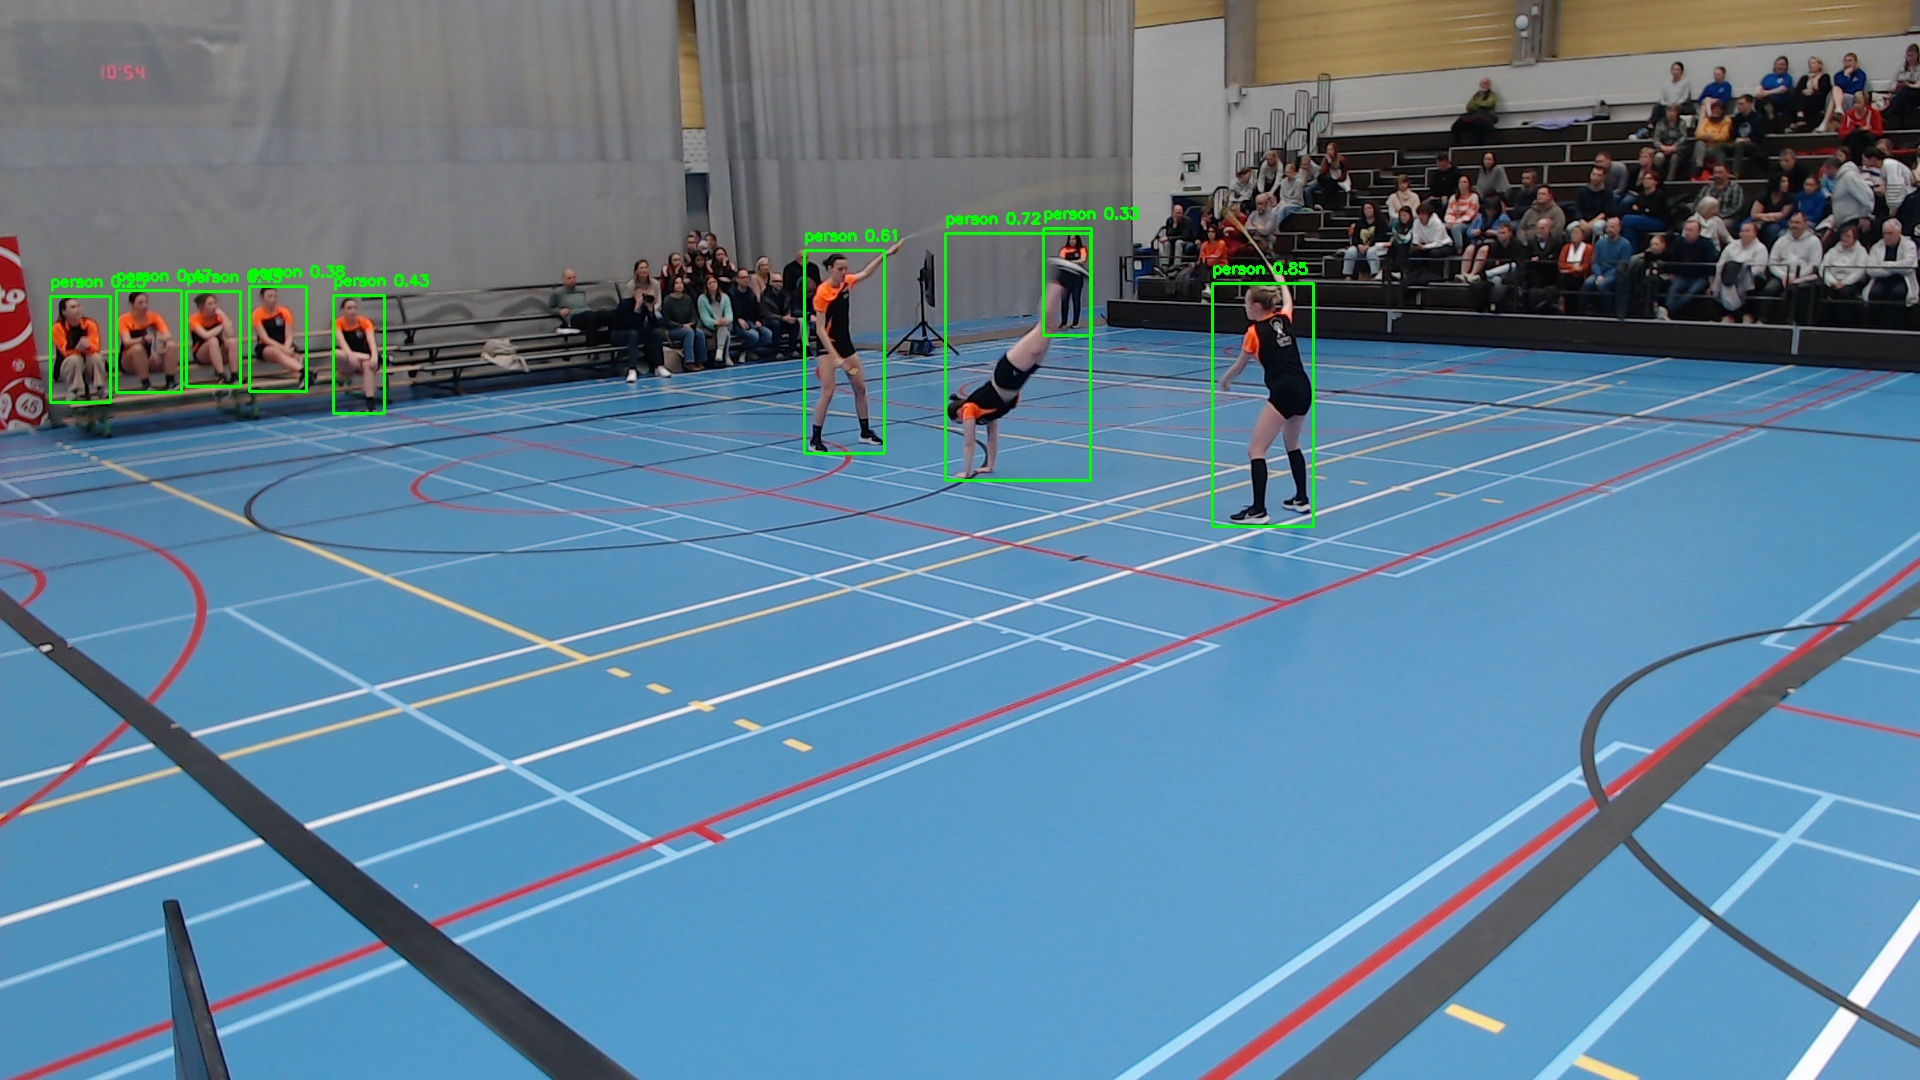
\includegraphics[width=0.95\linewidth]{1267_292_boxes}
    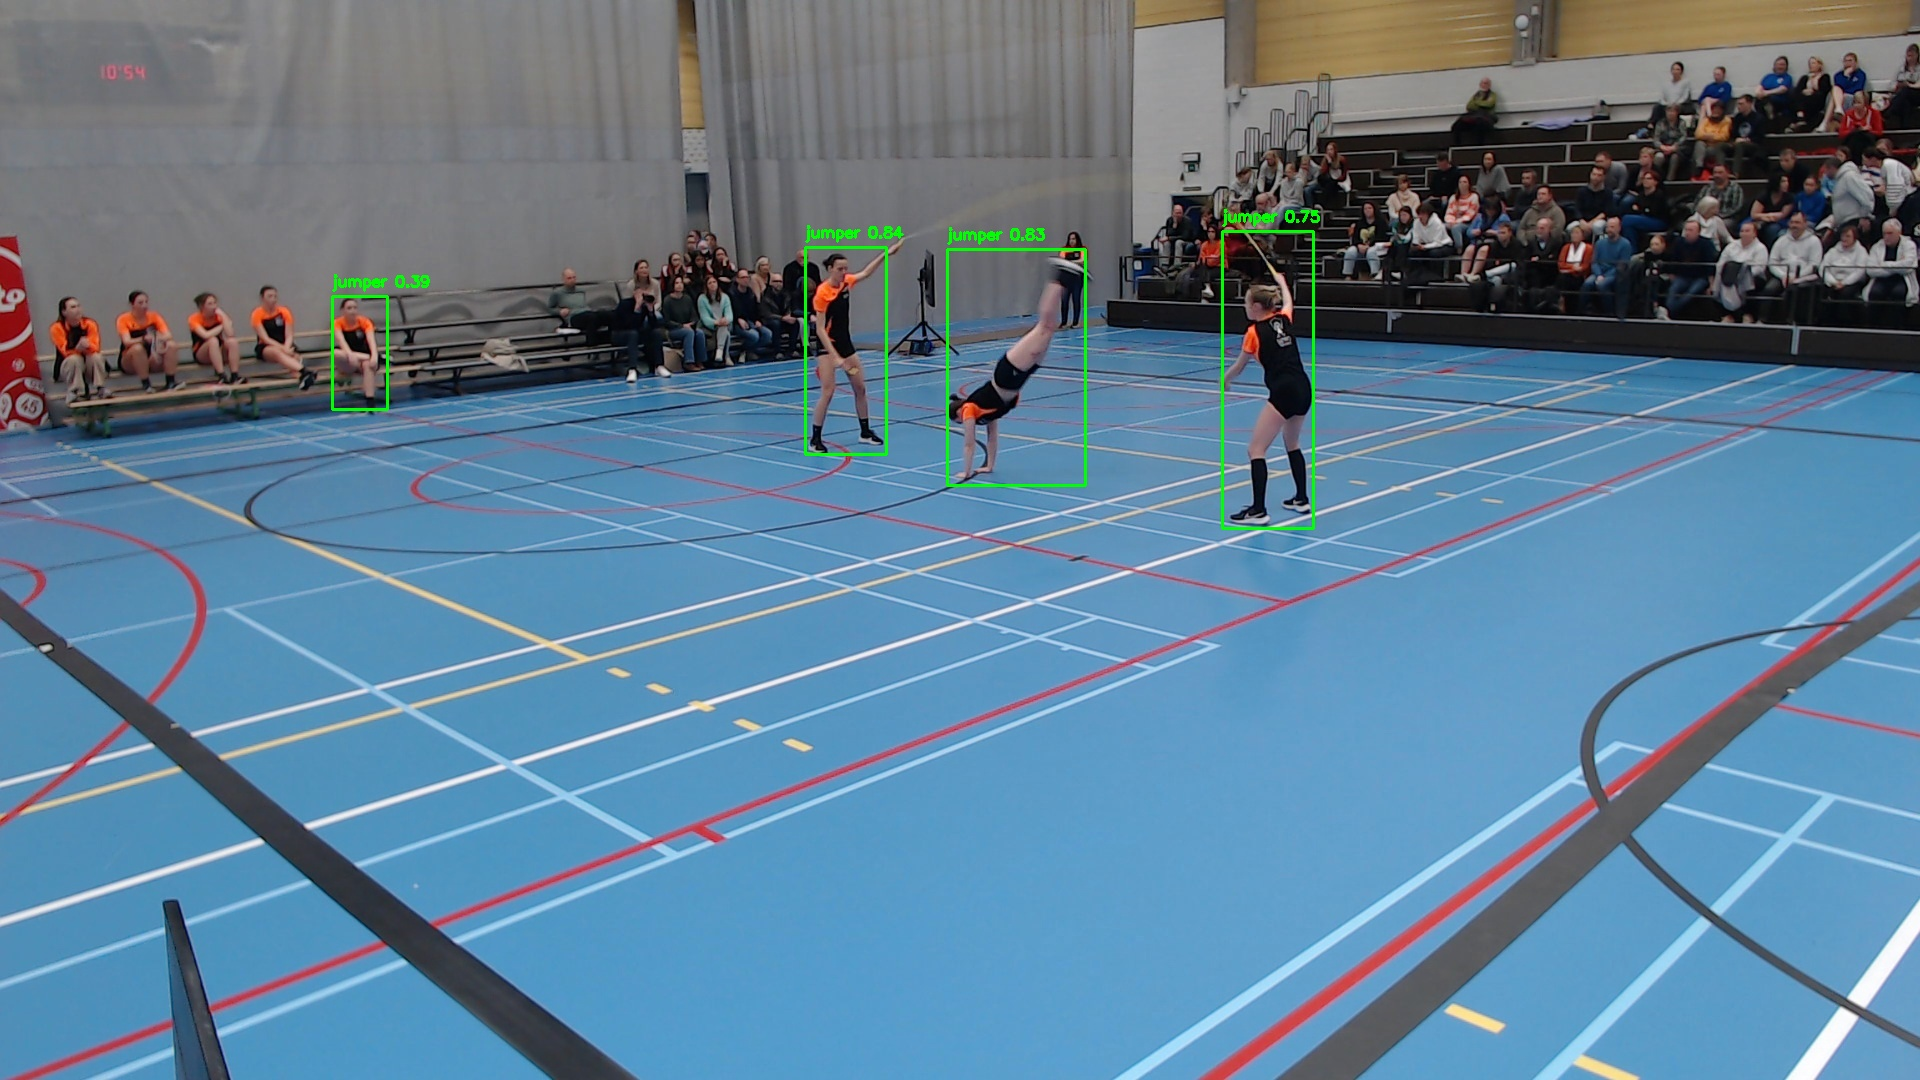
\includegraphics[width=0.95\linewidth]{1267_292_boxes_reduced_spectators}
    \caption[raw vs fine-tuned YOLOv11 nano model predictions]{Raw predictions of the unrefined YOLOv11 nano model compared to the fine-tuned model which reduces predictions of spectators.}
    \label{fig:raw-vs-fine-tuned-boxes}
\end{figure}

\begin{figure}
    \centering
%%    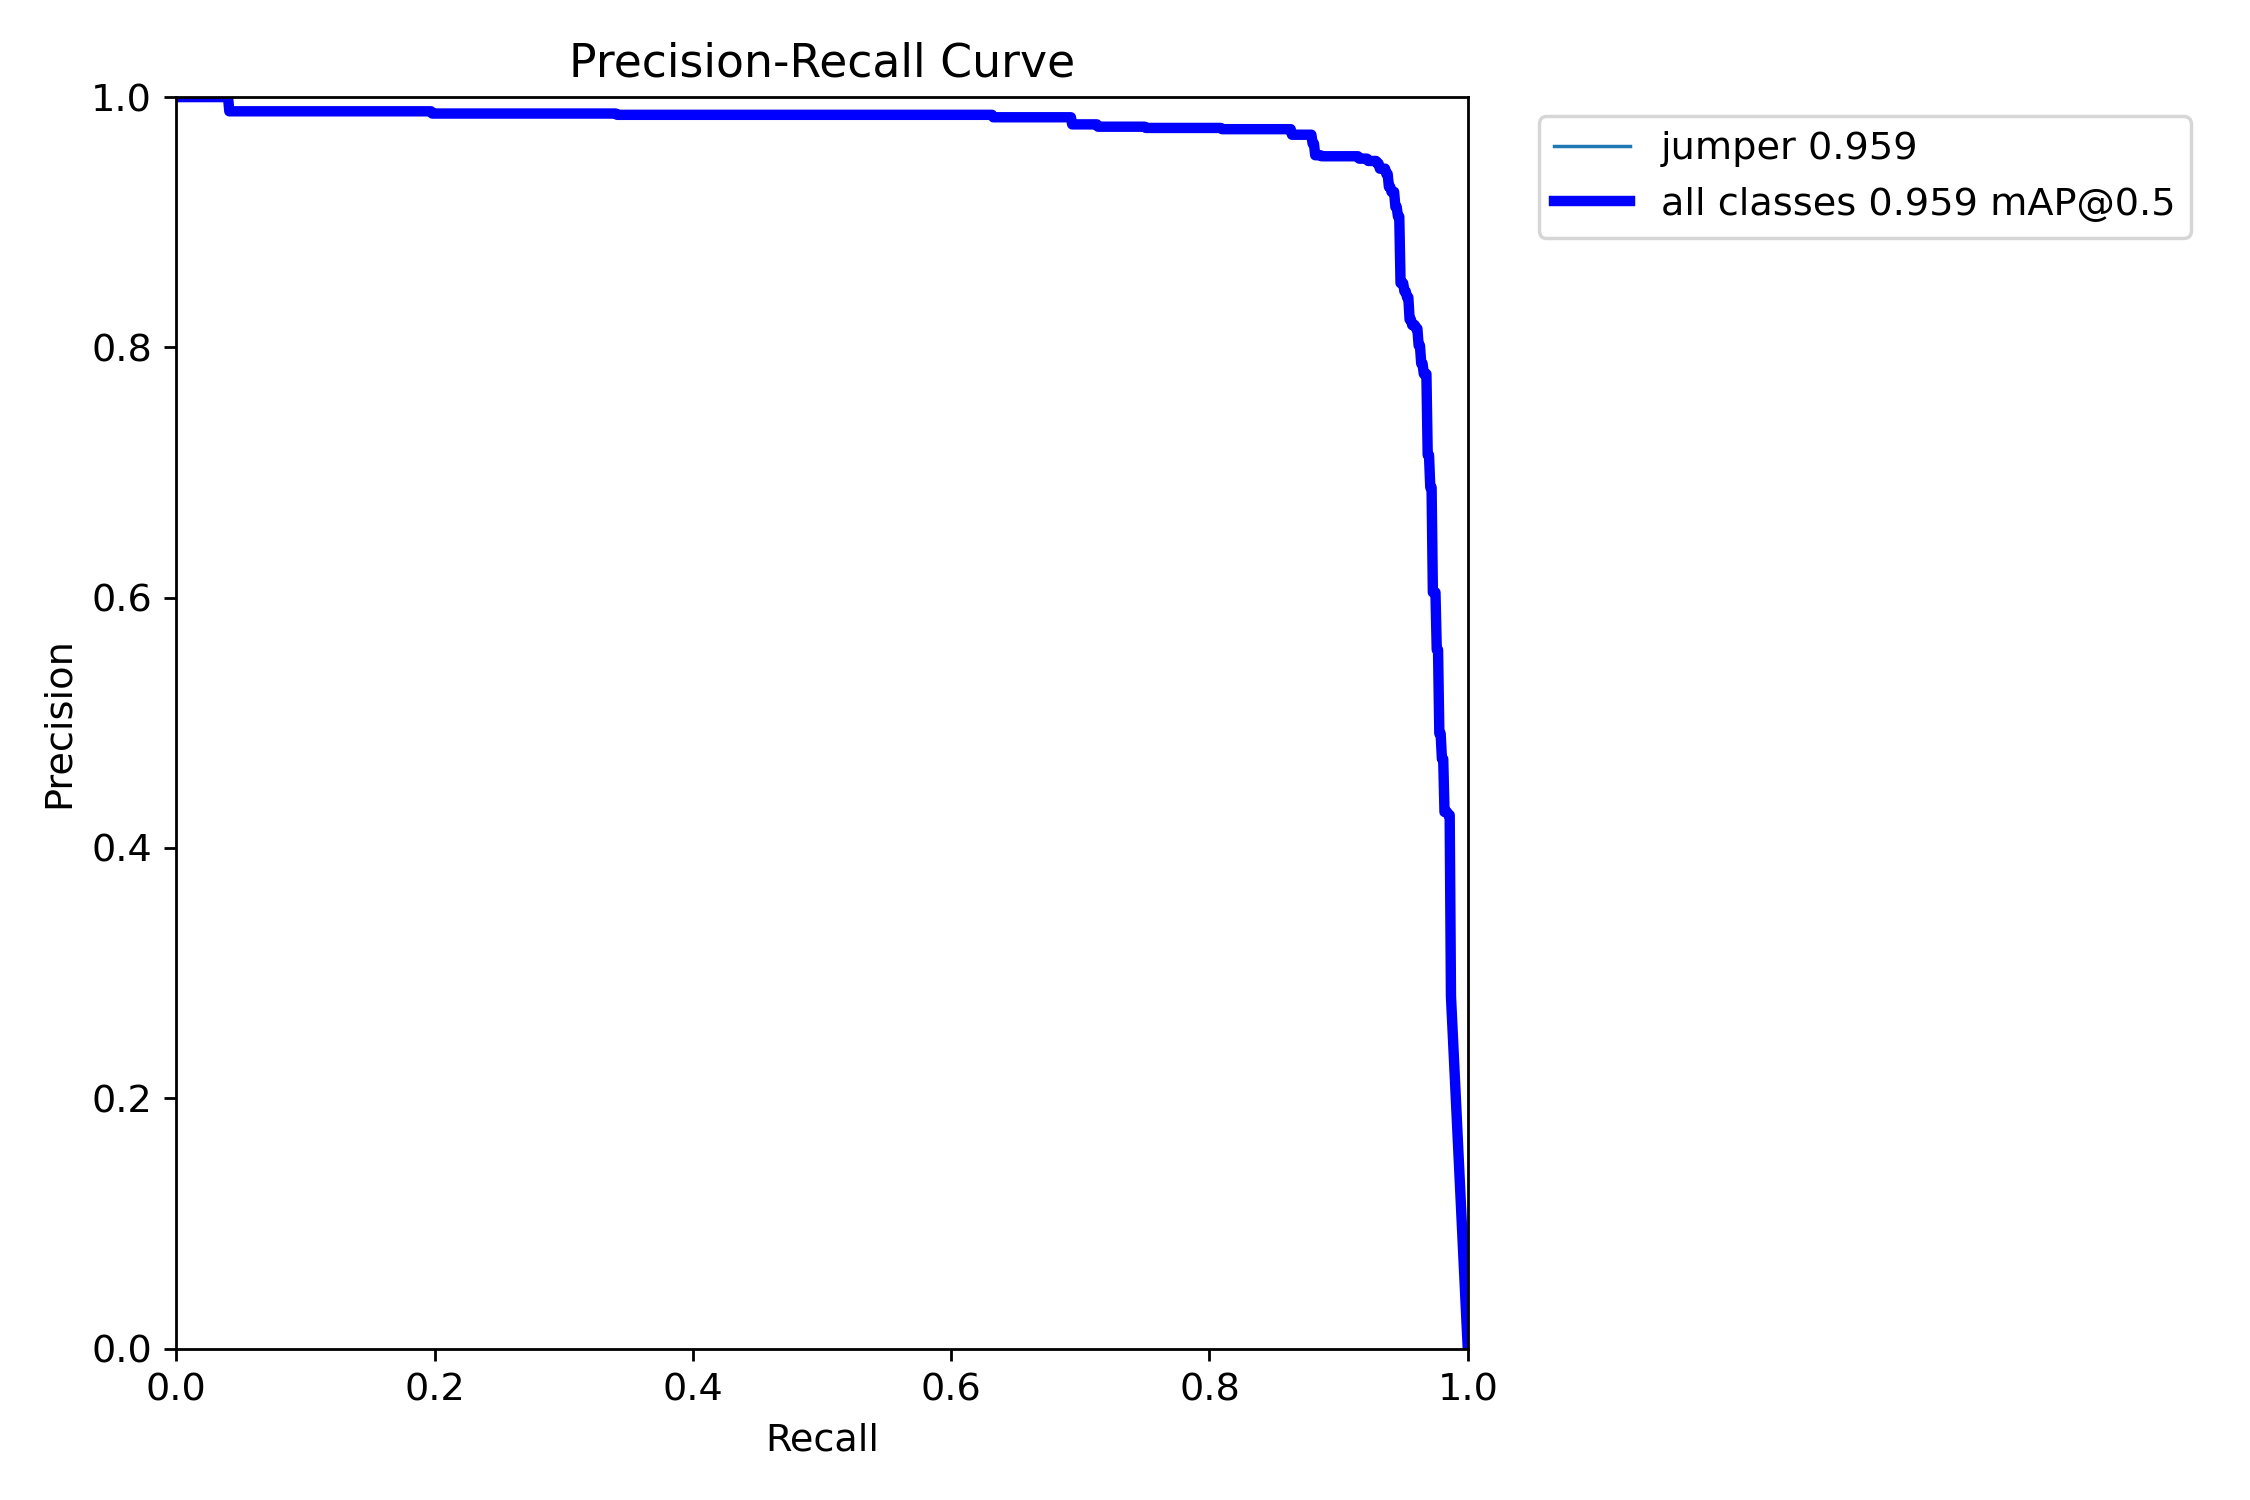
\includegraphics[width=0.35\linewidth]{PR_curve}
    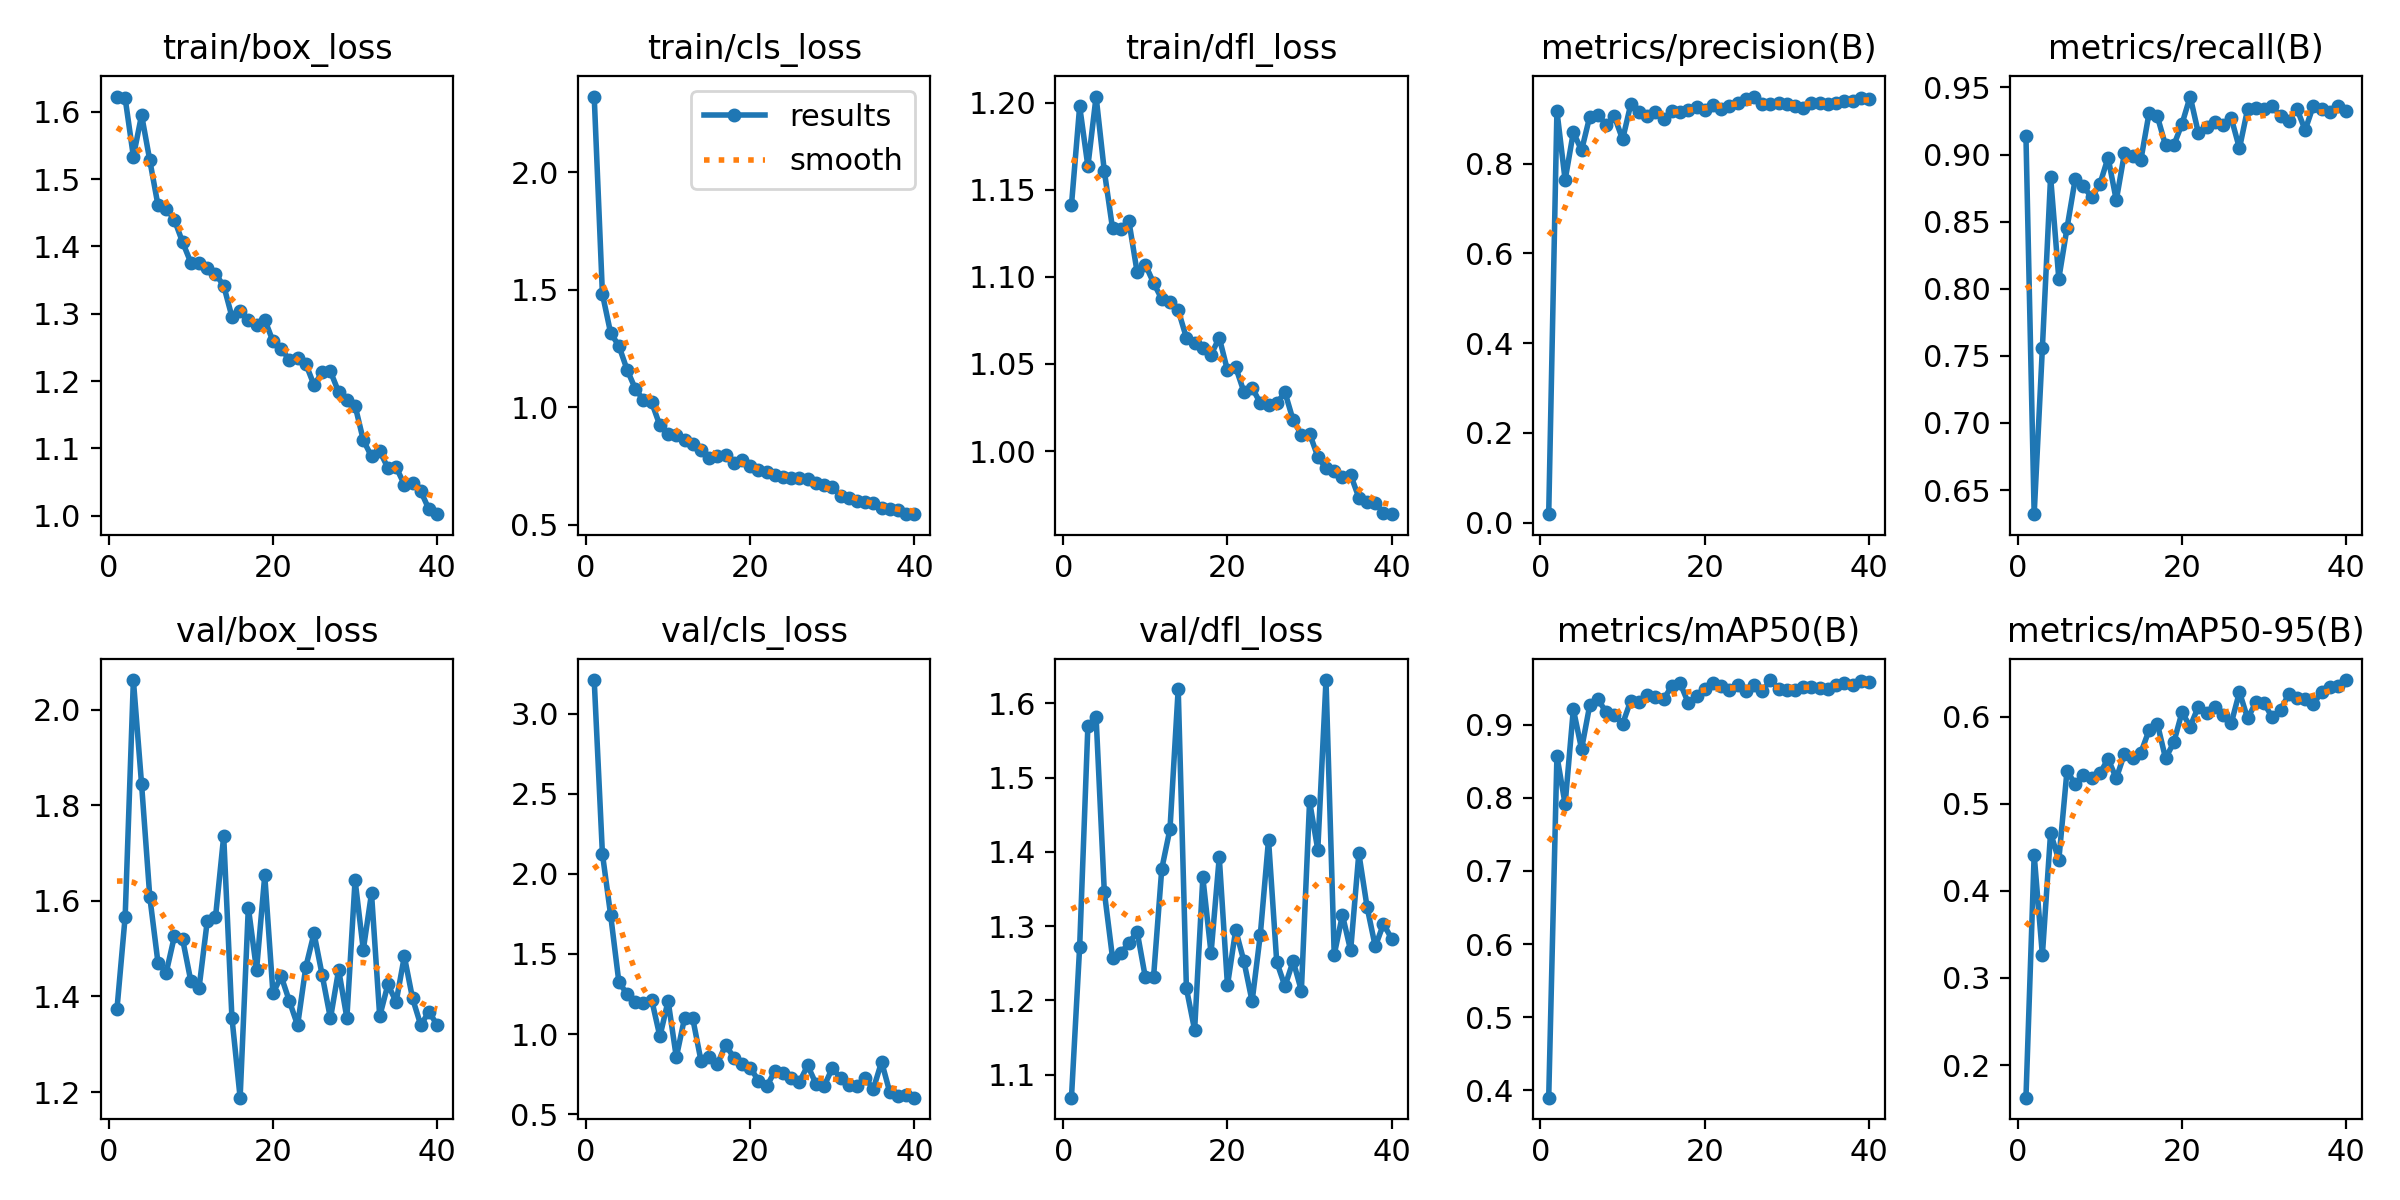
\includegraphics[width=0.95\linewidth]{results}
    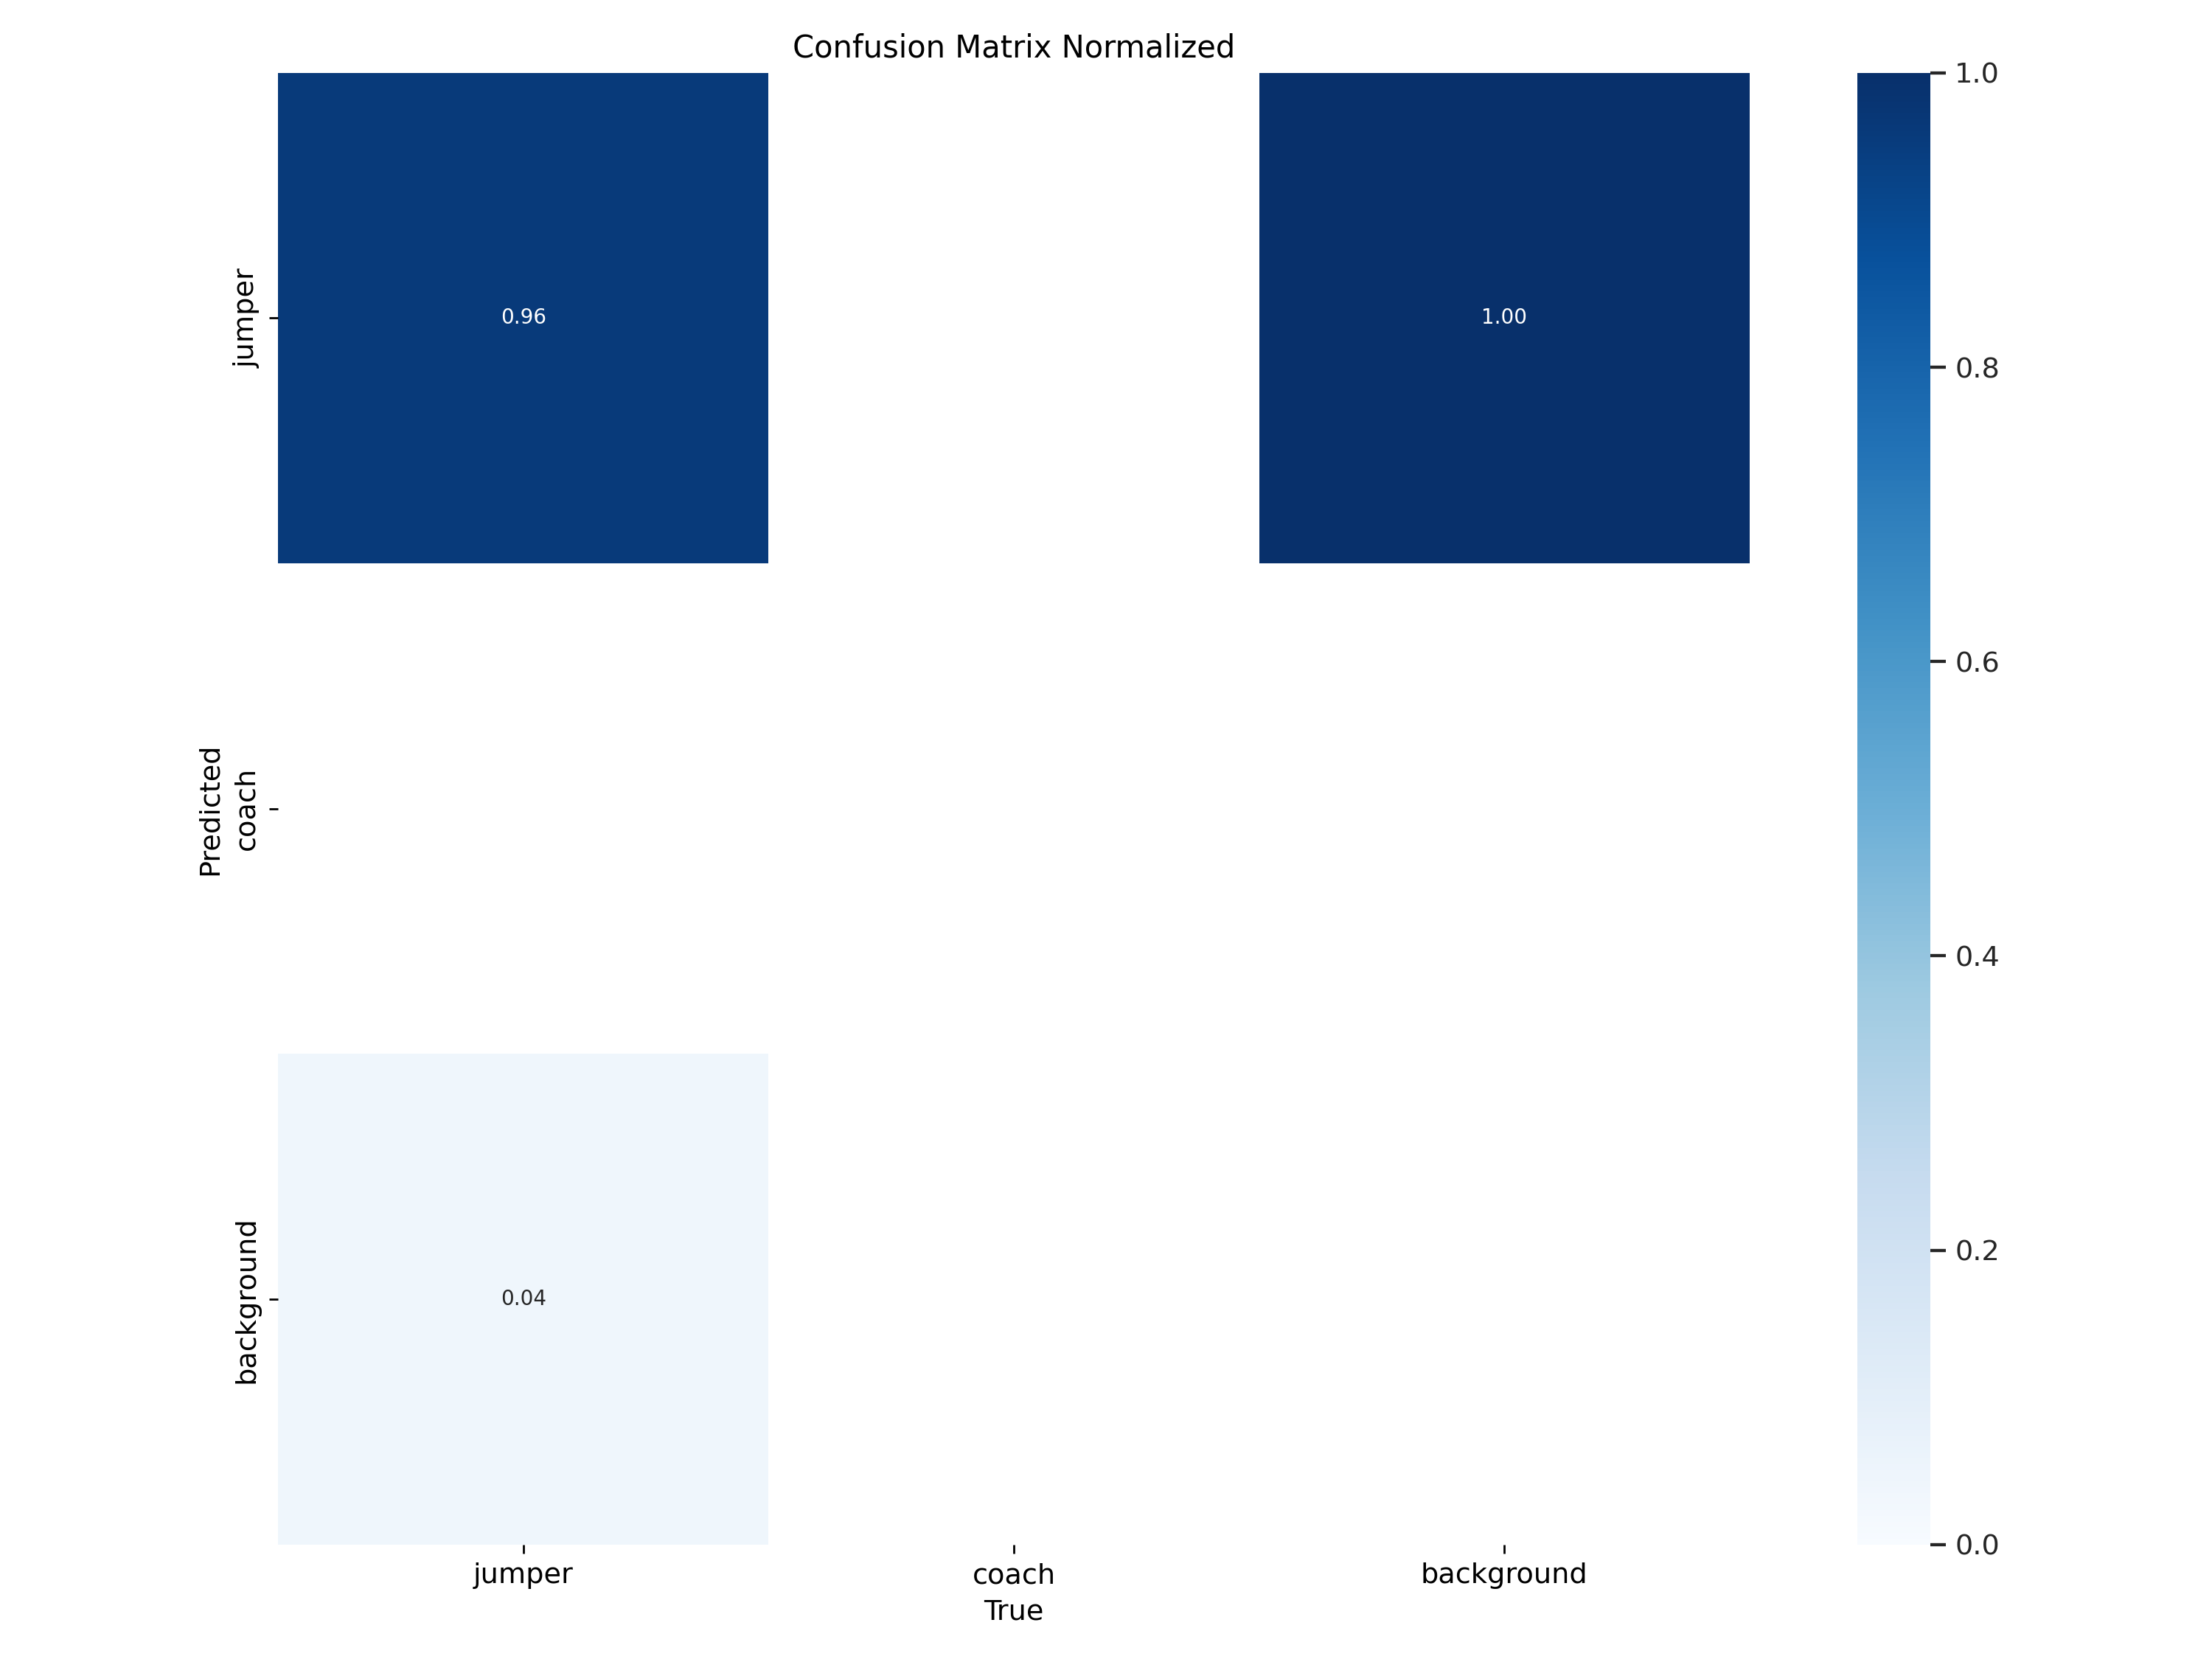
\includegraphics[width=0.85\linewidth]{confusion_matrix_normalized}
    \caption[metrics after fine-tuning YOLOv11]{Metrics after fine-tuning YOLOv11 on the validation set of 161 images, mAP50 of 0.953 \& mAP50-95 of 0.63, annotation of coaches was an idea.}
    \label{fig:localization-results}
\end{figure}

\begin{figure}
    \centering
    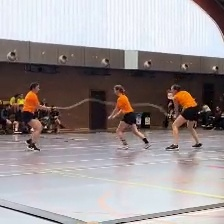
\includegraphics[width=0.45\linewidth]{1315_2935}
    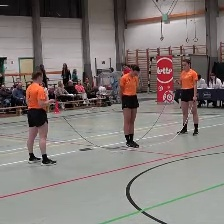
\includegraphics[width=0.45\linewidth]{2297_134}
    \caption[Valid crops of a DD3 routine on competition.]{Valid crops of a DD3 routine on competition. (224x224 pixels)}
    \label{fig:dd3-crop}
\end{figure}

\begin{figure}
    \centering
    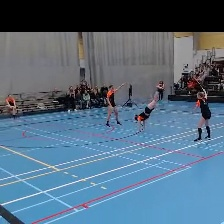
\includegraphics[width=0.45\linewidth]{1267_292_cropped}
    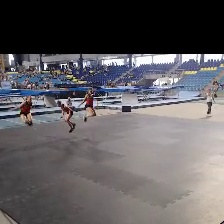
\includegraphics[width=0.45\linewidth]{1405_1061_cropped}
    \caption[dd3-crop-error]{Two crops including a spectator alongside the athletes.}
    \label{fig:dd3-crop-error}
\end{figure}

Annotating only athletes on 732 images \& fine-tuning the pre-trained nano yolo model, the first predictions of spectators are reduced considerately. This is illustrated in figure \ref{fig:raw-vs-fine-tuned-boxes}.
This way crops can be created by taking the minimum and maximum \(x\) \& \(y\)-coordinates of all boxes predicted on a frame. Predicting these crops for all frames, alles to crop a full video.
However, reviewing cropped videos indicate occasional frames predicting spectators, coaches or judges and moments of instability, as if you are watching camera footage of an earthquake.

In order to avoid a sudden zoom out, because of spectators, an IoU comparison of the previous predicted box with the new box is made. If the IoU value is larger than the average IoU of the last \(N\) seconds, powered to the fourth, than crop coordinates will be updated. Using this IoU comparison, reduces video crops including spectators, maintaining the earthquake effect.


To reduce shakiness and maintain a nice to watch cropped video, box-coordinates are smoothed out adapting box predictions of previous frames with the current one. This way, drastic changes in a predicted location, e.g. model error, arm or field movements aren't that drastic. Adaptation is done by incorporating two smooth values, indicating how much weight you give to the smoothed prediction of the previous frame. \footnote{Smoothed values are obtained by playing around with values, choosing those leading to the best, subjective, smoothed review}

$$ smth = smootval = 0.86  \quad \& \quad smths = smootval\_shrink = 0.94 $$

Which makes the new coordinates:

\bigskip
\begin{math}
   smooted_{x1_{min}} =
   \begin{cases}
       smooted_{x1_{min}} & \text{if} \quad iou < iou_{threshold} \\
       smth * smooted_{x1_{min}} + (1-smth) * x1_{min} & \text{else if} \quad x1_{min} < smooted_{x1_{min}} \\
       smths^ * smooted_{x1_{min}} + (1-smths) * x1_{min} & \text{otherwise}
   \end{cases}
\end{math}
\medskip

The same is done for \( y1_{min}, x2_{max}, y2_{max} \).

Utilizing these steps allows for videos where a team is always on display (\ref{fig:dd3-crop}), with some videos still predicting spectators (\ref{fig:dd3-crop-error}) and a newly introduced problem, namely skippers running out of view.

% TODO : add movement corrector

\begin{figure}
    \centering
    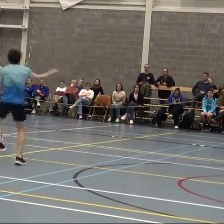
\includegraphics[width=0.45\linewidth]{1241_1093_cropped}
    \caption[dd3-crop-error]{Athletes running out of view.}
    \label{fig:dd3-crop-error-out-of-view}
\end{figure}

One way to solve jumpers running out of view, is by adding a default movement corrector, like the smooth value, which follows the new coordinates every frame. The movement corrector is based on the \(iou\)-value powered to the \(1/8\). It makes the crop following predictions by default, when IoU is getting low.

\medskip

\begin{math}
    SQRT = 8 \\
    movementCorrector = iou^{1/SQRT} \\
    smooted_{x1_{min}} = smooted_{x1_{min}} * movementCorrector + (1 - movementCorrector) * {x1_{min}}
\end{math}

\medskip

A possible improvement could be matching individual boxes with the new predictions, eliminating the spectator. Which raises concerns about jumpers entering the competition field. There are no earlier predicted boxes to match.
The total algorithm isn't perfect yet, but the results indicate sufficient valid video crops to use and experiment on segmentation and recognition \ref{code:localizor-with-strats}.

The results are broken down in table \ref{tbl:crop-results}. In this table you can see that about 15\% of the videos aren't localized properly, some of them only have minor disturbs. This results in enough videos available to try and recognize skills.

% TODO: pairwise distances?


% \subsection{Full video crops - automated testing (Work in Progress - WIP)}

% As manual checking videos can be time consuming, automated tests are in progress of creation in order to check whether crop strategies work or not.
% Utilizing the 7k legacy labels of full team boxes, video crops are calculated for each strategy.
% Both train and validation will be added separately in the results as there are less trainings videos labeled with individual boxes (129) than there are full box annotations on the trainings videos (325).
% The code for localizing has been cleaned as well. % (TODO add)








\section{Action segmentation}

Experiments on action segmentation have waited on skill recognition (section \ref{results:recognition}), this is why the experiments with action segmentation use the same models as the skill recognition, adapting only the top layers of the models.

\subsection{Video Vision Transformer \& Self-attention ConvLSTM}
\label{subsec:video-models-from-scratch}

The first and second experiment for segmention use code implementations of the Video Vision Transformer as introduced in \textcite{Arnab2021} (ViViT - \ref{code:get_model_ViViT}) and the Self-Attention ConvLSTM from \textcite{Lin_2020}.
To resolve bugs and dimensionality issues, Large Language models are used (\autocite{OpenAI_ChatGPT_2025} and \autocite{Deepseek_2025}).
These models were then trained on 7.8k batches of 16 consecutive frames, which originate from 44 trainings videos for about 48 minutes of training data, having framerates between 25 and 60 \footnote{Most labeled videos have a framerate of 25, 30 or 50 frames per second} images per second.
Both models showed the same results, averaging out predictions slightly above 0 for all frames, stagnating on MSE losses of around 0.09 and 0.10. This was about the average when always predicting 0. (Exact values are lost due to the switch to pytorch and bugs, will/could be re-added later.)

\subsection{Pre-trained MViT}
\label{results:action-segmentation-mvit}

In order to get better results on the little labeled available data, (44 videos for training, 7 validation videos), looking for a pre-trained model really helped a lot.
PyTorch provides a \href{https://pytorch.org/vision/main/models.html}{list} of pre-built and pre-trained models such as \href{https://pytorch.org/vision/main/models/video_mvit.html}{mvit-v1-b}.
Fine-tuning this model lowered the MSE to 0.065 with peaks overlapping splitpoints as demonstrated and elaborated in figure \ref{fig:segmentation-plot}.

To get all sections, all peaks in its neighborhood (\(windowsize = fps / 3\)) having a splitpoint value more than 0.4 become the start and end frame of a skill section, which will be used to recognize which skill is displayed. The code filtering segments out of raw-predicted splitpoint values is \ref{code:predictions-to-splitpoints}, filtering peaks (fig  \ref{fig:segmentation-plot}) in a list of start and end frames. An example could be \([...2280, 2320, 2355, 2382...]\), as splitpoints.


\begin{figure}
    \centering
    \includegraphics[width=0.45\linewidth]{segmentplot_2285_frameStart_2250_with_250_points}
    \includegraphics[width=0.45\linewidth]{segmentplot_2285_frameStart_2500_with_250_points}
    \includegraphics[width=0.45\linewidth]{segmentplot_2285_frameStart_2750_with_250_points}
    \includegraphics[width=0.45\linewidth]{segmentplot_2285_frameStart_3000_with_250_points}
    \caption[Segmentation plot]{Segmentation plot comparing predictions with the splitpoint values indicating a match of interesting splitpoint. Visible errors are: \\
        at frame 2459, a relatively lower jump out of the rope with a snapper. \\
        at frames 2700 until 2900 indicating a transition which is labeled in one segment, but the athletes are rather bouncy on their feet, letting the model think those are splitpoints. \\
        a handspring occurs from frame 3140 until 3192, but the model indicates too much during the skill, while it doesn't indicate the moment right after the handspring.
    }
    \label{fig:segmentation-plot}
\end{figure}

These predicted segments are the first usable split moments to use for splitting unseen videos recognizing or speeding up further labeling.
This brings us to the main results of this paper, namely skill recognition results.


\section{Skill recognition}
\label{results:skill-recognition}

\begin{figure}
    \centering
    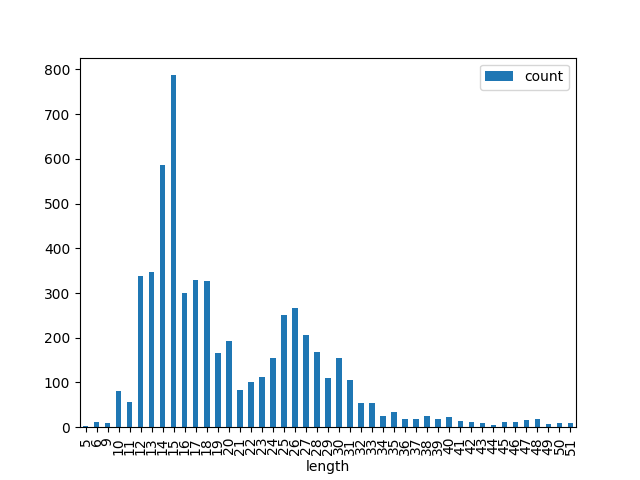
\includegraphics[width=0.95\linewidth]{skilllengths}
    \caption[frame counts of skill lengths]{Distribution of skill length (in frames), visually limited to 50 frames per skill. Skill lengths differ depending on the frame rate of the video. Most videos have a framerate of 25, 30 or 50 frames per second. Annotated sections longer than 50 frames are mostly transitions, mistake recoveries, gymnastic typed skills or powerskills with more than one rotation. These long duration frame counts occur at most 3 times.}
    \label{fig:skilllengths-counts}
\end{figure}


Having small little sections of potential skills (normal jumps, and mistake recoveries included) allows to predict what actions are actually in this section.
As the segments provided by the segmentation model have a varying frame count, and the length of skills in general can differ, they need to be transformed in equal sized frames.
Depending on the frame rate, most skills have a frame rate between 12 and 18 frames per skill, see figure \ref{fig:skilllengths-counts} for a distribution. In order to transform skills into equally sized sections, frames are skipped or duplicated depending on the length of the skill.
The selected frames are calculated in code snippet \ref{code:skill-frame-selection}.


\begin{listing}
    \begin{minted}{python}
        timesteps = 16
        slot = skill_length_over_timesteps = skill_length / timesteps
        frames [frames_skill[round(i * slot)] for i in range(timesteps)]
    \end{minted}
    \caption[Code for frame selection skills]{Code for frame selection of skills}
    \label{code:skill-frame-selection}
\end{listing}



\subsection{Video Vision Transformer \& Self-attention ConvLSTM}

Using about 5k skills, 4550 to train and 669 to validate, the same video models as described in the segmentation phase \ref{subsec:video-models-from-scratch} can be trained the skill properties defined in \ref{lit:skill-matrix}.
During the annotation of videos, it is noticed how screwed the skill-data is. Other action properties like turners, hands, type or faults are equally skewed. See table \ref{tab:skill_distribution_full_with_nulls} for a breakdown of skill occurrences.

Both the ViViT and the SA-ConvLSTM were plateauing on the most appearing value, always predicting normal jumps, normally turned, without a mistake etc.
Even up-sampling less occurring combinations didn't help. The models stagnated on validation losses of 5.9 and 6.5. See figure \ref{fig:skill-upsampling-distribution} to see how many times a skill appears in a training round, depending on its uniqueness.

\begin{figure}
    \centering
    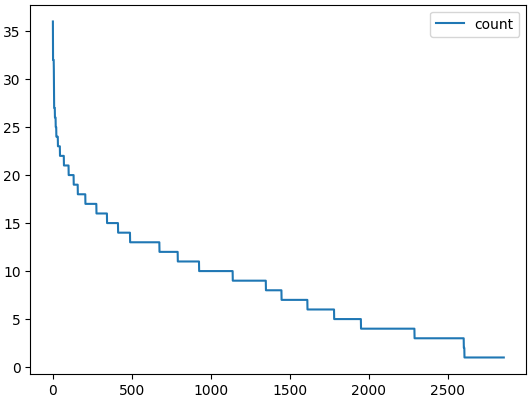
\includegraphics[width=0.7\linewidth]{skill-upsampling-distribution}
    \caption[upsampling distribution of skills]{Occurance of each labeled skill (e.g. videoId 123, frameStart 480, frameEnd 504, Double Dutch, 1 rotation, split, EB, crouger...) in the upsampeled dataset. Values get duplicated based on the uniqueness of each property. E.g. because it is an EB and a split, it will be duplicated four times, but no/less duplication because Double Dutch and 1 rotation is more common.}
    \label{fig:skill-upsampling-distribution}
\end{figure}

In order to reach better results, the search for a pre-trained model leads us to the following experiment, namely the usage of PyTorch implementation of the Multiscale Video Vision Transformer.

\subsection{Multiscale Video Vision Transformer - MViT}
\ref{results:mvit}

The implementation of the the Mutliscale vision transformer uses the PyTorch pre-trained model and weights \ref{code:pytorch-mvit-init}.
The output layers of the model are stripped in order to adapt the model to recognizing jump rope skills. This allows the addition of new output layers, custom to DD3 freestyles \ref{code:pytorch-skill-output-layers}.

\begin{figure}
    \centering
    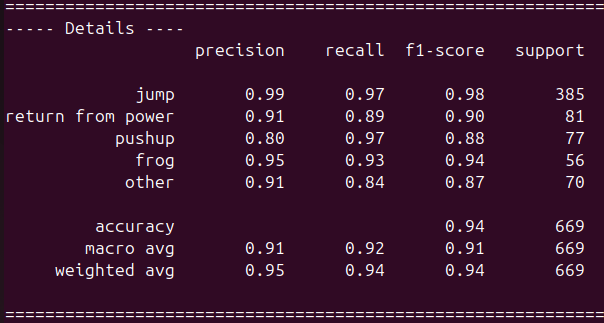
\includegraphics[width=0.7\linewidth]{mvit-5-classes}
    \caption[Classification report on only 5 skill classes]{Classification report on the 5 classes jumps, pushups, return from powers, frogs or other skills after training mvit on an equally distributed, max 442 samples per skill as seen in table \ref{tab:skill_distribution_grouped_final}.}
    \label{fig:mvit-5-classes}
\end{figure}


\href{https://pytorch.org/vision/main/models/video_mvit.html}{PyTorch's Video MViT} is an implementation based on the Multiscale Vision Transformer created by \textcite{Fan2021} which can be finetuned using the pre-trained weights on the kinetics dataset.
The first experiment using this model used a perfectly balanced dataset for skills only, namely taking a random subset of maximum of 442 samples on each of the 5 classes seen in table \ref{tab:skill_distribution_grouped_final}.
The first results showed accuracies of 87\% to 98\% (see fig. \ref{fig:mvit-5-classes}) even some turner skills getting predicted correctly.

Re-enabling all skill classes and all other properties results in a total validation loss of 1.3835, as compared to 5.9 or 6.5 earlier.
For skills only, the weighted f1-accuracy is 93\%, while macro f1-accuracy is 40\%.
The macro accuracy gives a better indication as accuracies on all defined classes, e.g. pushup, jump, swift, are taken into account equally. In this experiment, the less appearing skills lower the score of the macro accuracy, as they do not appear as often.

Like the previous subsection, these results are trained on the skill distribution displayed in table \ref{tab:skill_distribution_full_with_nulls}).
A breakdown of all classification reports can be found in tables \ref{tbl:mvit-first-class-reports-type} -> \ref{tbl:mvit-first-class-reports-fault}. You may notice that the predictions for bodyRotations, sloppy, hard2see \& faults have yet to start learning.

\begin{table}[h!]
    \centering
    \begin{tabular}{|r|r|l|r|r|}
        \hline
        \textbf{Train \%} & \textbf{Train Count} & \textbf{Skill} & \textbf{Val Count} & \textbf{Val \%} \\
        \hline
        50.6687 & 2273 & jump & 379 & 56.6517 \\
        14.0660 & 631 & pushup & 77 & 11.5097 \\
        13.0629 & 586 & return from power & 84 & 12.5561 \\
        9.8529 & 442 & frog & 59 & 8.8191 \\
        3.2100 & 144 & crab & 9 & 1.3453 \\
        2.0062 & 90 & split & 12 & 1.7937 \\
        1.1146 & 50 & flip & 5 & 0.7474 \\
        0.9140 & 41 & rondat & 5 & 0.7474 \\
        0.8917 & 40 & rad & 3 & 0.4484 \\
        0.8025 & 36 & suicide & 8 & 1.1958 \\
        0.7356 & 33 & handspring & 5 & 0.7474 \\
        0.6910 & 31 & rol2kip & 7 & 1.0463 \\
        0.4458 & 20 & kip & 6 & 0.8969 \\
        0.3567 & 16 & speed & NULL & NULL \\
        0.3121 & 14 & kopkip & 1 & 0.1495 \\
        0.2675 & 12 & roll & 3 & 0.4484 \\
        0.1783 & 8 & stut & 2 & 0.2990 \\
        0.1337 & 6 & swift & NULL & NULL \\
        0.1337 & 6 & UNKOWN & 1 & 0.1495 \\
        0.0669 & 3 & leapfrog & NULL & NULL \\
        0.0446 & 2 & footwork-kick & NULL & NULL \\
        0.0223 & 1 & mountainclimber & NULL & NULL \\
        0.0223 & 1 & footwork-open & 1 & 0.1495 \\
        \hline
    \end{tabular}
    \caption[Skill distribution skill]{Skill distribution with training and validation counts and percentages. Null values indicate absence of skill occurrence in the validation data.}
    \label{tab:skill_distribution_full_with_nulls}
\end{table}


\begin{table}[h!]
    \centering
    \begin{tabular}{|l|r|r|r|r|}
        \hline
        \textbf{Skill} & \textbf{Train Count} & \textbf{Train \%} & \textbf{Val Count} & \textbf{Val \%} \\
        \hline
        jump & 2273 & 50.6687 & 379 & 56.6517 \\
        pushup & 631 & 14.0660 & 77 & 11.5097 \\
        return from power & 586 & 13.0629 & 84 & 12.5561 \\
        frog & 442 & 9.8529 & 59 & 8.8191 \\
        other & 526 & 11.7253 & 68 & 10.1645 \\
        \hline
    \end{tabular}
    \caption[Skill distribution skills limited classes]{Train and validation skill distribution with low-frequency skills grouped as "other"}
    \label{tab:skill_distribution_grouped_final}
\end{table}

\subsection{Skill recognition - Act as a judge}
\label{results:skill-recognition-act-as-a-judge}

Being able to recognize skills allows to assign respective levels on combinations. After assigning the proper levels, the respective scores can be assigned mapping based on the total levels jumped. Table \ref{tbl:Score mapping} illustrates how many points each level receives.

The first results are shown using recordings of national finals. With an average score difference of -32.17\%. The first score mappings don't look that good.
Inspecting these results further, some videos indicate more than -70\% score difference. Inspecting these results show invalid crops predicting spectators, potentially because of a different sport gymnasium and a lower camera perspective, compared to other videos.
Another competition will be put next to these results, in order to gain more insights.
% TODO : side note, herhalingen zijn er nog niet eens uit.

\begin{table}
    \begin{tabular}{|l|l|}
        \hline Level & Score \\ \hline
        0 & 0 \\
        1 & 1.5 \\
        2 & 2.2 \\
        3 & 3.3 \\
        4 & 4.9 \\
        5 & 7.3 \\
        6 & 11 \\
        7 & 11 \\
        8 & 11 \\ \hline
    \end{tabular}
    \caption[level to score map]{Corresponding score for each skill level, in Belgium, levels are limited to 6, any higher level remains a level 6. (Applicable during seasons 2023-2024 and 2024-2025)}
    \label{tbl:Score mapping}
\end{table}

\begin{table}[h!]
    \begin{tabular}{|l|r|r|r|}
        \hline
        videoId & judges    & MViT         & Differencs \\ \hline
        2568	& 169.26	&   147	       & -13.15 \\
        2569	& 181.23	&   166.9	   & -7.91  \\
        2570	& 146.71	&   25.4	   & -82.69 \\
        2571	& 180.58	&   170.8	   & -5.42  \\
        2572	& 251.14	&   68.7       & -72.64 \\
        2573	& 141.37	&   9.7	       & -93.14 \\
        2574	& 272.28	&   227.4	   & -16.48 \\
        2575	& 331.22	&   257.9	   & -22.14 \\
        2576	& 210.86	&   207.3	   & -1.69  \\
        2577	& 261.63	&   130.9	   & -49.97 \\
        2578	& 128.6	    &   135.6	   & +5.44  \\
        2579	& 203.48	&   196.4	   & -3.48  \\
        2581	& 216.81	&   89.6	   & -58.67 \\
        2582	& 259.88	&   223.7	   & -13.92 \\
        2583	& 348.27	&   168.4	   & -51.65 \\
        2584	& 366.94	&   177 	   & -51.76 \\
        2585	& 68.31	    &   54.6	   & -20.07 \\
        2586	& 175.59	&   159.9	   & -8.94  \\
        2587	& 260.29	&   192.1	   & -26.2  \\
        2588	& 319.09	&   231.4	   & -27.48 \\
        2589	& 148.5	    &   108 	   & -27.27 \\ \hline
        Total   & 4642.04	&   3148.7	   & -32.17 \\ \hline
    \end{tabular}
    \caption[judge diff score compared to MViT]{Score assigned by judges compared to the prediction the MViT model \\
    Videos are on fully unlabeled data and from the same competitionday, with a camera perspective quite a bit lower than other times.
    This results in quite some videos with inproper crops.}
    \label{tbl:judge-score-comparison}
\end{table}

\subsection{Weighted loss}
\label{results:skill-recognition-weighted-loss}

% TODO : paper source?
In order to increase accuracy on lower represented classes. To enforce this, losses wil be increased for mistakes on lower represented classes. A little mathematical magic \ref{code:recognition-weighted-loss} based on the value counts of each skill aspect compared to highest occurance, applying some buffer, taking the difference, squaring, comparing to the mean etc. (\ref{code:recognition-weighted-loss}) allows for weight distributions below.

\begin{itemize}
    \item loss weights for Type [1.0000, 1.5151, 4.7846, 4.7938, 4.2562, 4.7383, 4.6330]
    \item loss weights for Rotations [4.4372, 1.4893, 3.9782, 4.4880, 4.5276, 4.5960, 4.5960, 4.0000, 4.5997]
    \item loss weights for Turner1 [1.0000, 1.4437, 3.8602, 3.6128, 4.1699, 4.1746, 4.1079, 4.1067, 4.1866, 4.1711, 4.1818, 4.1818, 4.1890, 4.1902, 4.1878, 4.1926, 4.0000, 4.1914, 4.1914, 4.1938, 4.0000, 4.1926, 4.1902, 4.1938, 4.1938, 4.1938, 4.1938]
    \item loss weights for Turner2 [1.0000, 1.4450, 3.8687, 3.6231, 4.1794, 4.1890, 4.1026, 4.1325, 4.1938, 4.1866, 4.1854, 4.1926, 4.1926, 4.1986, 4.1950, 4.2023, 4.2023, 4.1974, 4.1986, 4.0000, 4.2011, 4.2011, 4.1998, 4.0000, 4.2035, 4.0000, 4.1998]
    \item loss weights for Skill [1.0000, 1.4673, 2.5125, 2.5218, 2.5897, 4.0175, 4.4216, 3.8261, 4.4017, 4.4216, 4.2631, 4.2532, 4.2697, 4.3224, 4.3752, 4.2236, 4.4216, 4.2828, 4.3719, 4.4150, 4.2598, 4.4216, 4.4183, 4.3786, 4.4183, 4.3719, 4.4183, 4.0000, 4.0000, 4.0000, 4.3984, 4.4216, 4.4216]
    \item loss weights for Hands [2.0090, 7.7774, 3.2177]
    \item loss weights for Feet [5.6549, 5.2853, 1.7504]
    \item loss weights for Turntable [1.6041, 5.5475, 5.6556]
    \item loss weights for BodyRotations [1.5966, 5.6104, 5.6066]
    \item loss weights for Backwards [1.7598, 7.1472]
    \item loss weights for Sloppy [1.7704, 7.1258]
    \item loss weights for Hard2see [1.7622, 7.1423]
    \item loss weights for Fault [1.7756, 7.1154]
\end{itemize}

These weights are then given to CrossEntropyLoss of PyTorch for the categorical outputs and given to a customized MSE \ref{code:weighted-mse}, for numerical and boolean outputs, incorporating these weights.
This resulted for Faults, Sloppy and Hard2See to start being recognized \ref{tbl:mvit-class-reports-fault-after-weighted-losses} and pushed the total macro f1 avg accuracy to 51.53\%, which is about 6\% higher then before.

\section{Video ResNet and Swin Transformer}
\label{results:skill-recognition-resnet-swin-saconv3d}

To top it all, additional models where added to fully compare the performance of the MViT model.
The first additions are the PyTorch implementation of video ResNet models, based on the paper of \textcite{Tran2017}.
All three of the adaptions, R3D, MC3 and R2plus1 were stripped from their head and filled with the jump rope skill output layers, just like the MViT implementation. Another model listed by PyTorch was the Swin Transformer, created by \textcite{Liu2021}, implemented the same way. Only the tiny (t) and small (s) versions of the Swin transformer have been tested.

Utilizing the pre-trained weights on kinetics 400, only the Swin Transformer reached similar results and even bested the Multiscale Vision Transformer by a few percentiles (52.36\%), which you can see in table below \ref{tbl:skill-recognition-model-comparison}.
However, the MViT models stays strong, keeping the highest total accuracy (93.83).
% The final model which is implemented, not using pytorch

\begin{table}[h!]
    \begin{tabular}{|l|r|r|r|r|r|}
        \hline model &  macro & m skills & weighted & w skills & total accuracy \\ \hline
        Resnet\_R2plus1	    & 25.64 &	2.70 &	70.3	& 25.51	& 71.87 \\
        Resnet\_MC3	        & 25.98 &	1.39 &	69.49	& 9.85	& 69.88 \\
        Resnet\_R3D	        & 27.43 &	3.52 &	70.24	& 19.76	& 71.22 \\
        SwinT\_t	        & 49.13 &	32.06 &	91.28	& 89.4	& 91.99 \\
        MViT	            & 51.53 &	27.75 &	93.11	& 90.7	& 93.83 \\
        MViT\_extra\_dense	& 51.96 &	31.46 &	93.1	& 91.45	& 93.73 \\
        SwinT\_s	        & 52.36 &	36.73 &	92.8	& 91.79	& 93.3  \\ \hline
\end{tabular}
\caption[Skill recognition comparison on multiple models]{
    macro = f1 avg macro accuracy \\
    m skills = f1 avg skill accuracy \\
    weighted = f1 weighted avg \\
    w skills = f1 weighted avg skills \\
    total accuracy = true positives / total aspects
}
\label{tbl:skill-recognition-model-comparison}
\end{table}

% SA_Conv3D	        & 24.12 &	2.53 &	69.71	& 37.97	& 75.39 \\

Using these increased accuracies on recognition \& other models, judge scores can be compared along the models.
To keep things uncluttered, only the total deviation is showed now. While the swin transformers showed more potential in the macro recognition of skills, the multiscale video transformer outperformed on similarity with the judges.

\begin{table}[h!]
    \begin{tabular}{|r|r|r|r|r|r|r|}
        \hline
        MViT   & MViT dense  & Swin s & Swin t & MC3    & R3D   & R2plus1 \\ \hline
        -21.68 & -20.94      & -23.83 & -27.72 & -38.85 &-53.09 & +47.15  \\ \hline
    \end{tabular}
    \caption[Judge diff score compared to all models]{Score assigned by judges compared to the prediction vision models \\
    The multiscale vision transformer is clearly winning on assigning scores.}
    \label{tbl:judge-score-comparison}
\end{table}

You may have noticed, that the final run decreased the score difference from -32.17\% to a whopping -21.68\%, finalizing the results in a positive note, being able to discuss and summarize this research.